\SourceLeaf{230}%
\Needspace{27\baselineskip}
V. Lehrsatz. Es ist allgemein $f\varphi+f\psi+f(180^{0}-\varphi-\psi)=t$.

Der Beweis erhellt leicht aus der Figur, wo die drei Flächentheile $\underline{1,\,2,\,3}$ die Werthe haben
\[
\begin{aligned}
\underline{1}&=f(180^{0}-\varphi-\psi),\\
\underline{2}&=f\varphi,\\
\underline{3}&=f\psi
\end{aligned}
\]
und ihre Summe $=t$ wird.
\begin{center}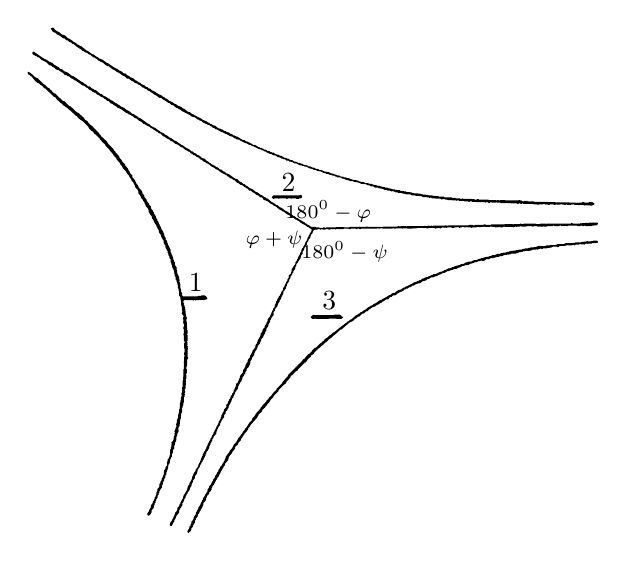
\begin{tikzpicture}[x=0.00543718cm,y=-0.00543718cm]
\fill[even odd rule] (667,685) -- (667,687) -- (671,690) -- (675,690) -- (676,689) -- (678,689) -- (679,690) -- (708,690) -- (709,689) -- (727,689) -- (728,690) -- (732,690) -- (734,689) -- (735,690) -- (738,690) -- (742,687) -- (742,686) -- (735,680) -- (722,680) -- (721,681) -- (675,681) -- (673,680) -- cycle
(1338,509) -- (1336,507) -- (1327,507) -- (1326,508) -- (1322,508) -- (1321,509) -- (1312,508) -- (1311,509) -- (1300,510) -- (1299,511) -- (1286,511) -- (1285,512) -- (1278,512) -- (1277,513) -- (1262,513) -- (1259,515) -- (1244,515) -- (1240,517) -- (1218,518) -- (1214,520) -- (1204,520) -- (1203,519) -- (1199,519) -- (1193,522) -- (1180,523) -- (1179,524) -- (1176,524) -- (1175,525) -- (1168,525) -- (1167,526) -- (1163,526) -- (1160,528) -- (1153,528) -- (1152,529) -- (1147,529) -- (1146,530) -- (1134,531) -- (1133,532) -- (1131,532) -- (1130,533) -- (1126,533) -- (1122,535) -- (1117,535) -- (1116,536) -- (1112,536) -- (1108,538) -- (1103,538) -- (1099,540) -- (1091,541) -- (1088,543) -- (1085,543) -- (1084,544) -- (1073,546) -- (1069,548) -- (1065,548) -- (1064,549) -- (1062,549) -- (1055,552) -- (1047,553) -- (1042,556) -- (1036,556) -- (1032,558) -- (1029,558) -- (1025,561) -- (1021,561) -- (1020,562) -- (1018,562) -- (1017,563) -- (1003,567) -- (1000,569) -- (997,569) -- (995,571) -- (988,572) -- (983,575) -- (980,575) -- (978,577) -- (974,579) -- (969,580) -- (959,585) -- (954,585) -- (952,587) -- (950,587) -- (945,590) -- (943,590) -- (940,592) -- (937,592) -- (929,596) -- (927,596) -- (924,599) -- (922,599) -- (919,601) -- (917,601) -- (914,603) -- (907,605) -- (903,608) -- (888,615) -- (886,617) -- (883,617) -- (878,621) -- (871,623) -- (869,625) -- (866,626) -- (863,629) -- (860,629) -- (856,631) -- (854,633) -- (847,636) -- (844,639) -- (842,639) -- (840,641) -- (835,643) -- (833,645) -- (827,647) -- (819,653) -- (814,655) -- (811,658) -- (809,658) -- (805,661) -- (802,662) -- (795,668) -- (789,671) -- (786,674) -- (784,674) -- (781,677) -- (778,678) -- (776,680) -- (772,682) -- (763,690) -- (759,692) -- (756,695) -- (753,696) -- (749,700) -- (748,700) -- (745,703) -- (740,706) -- (723,720) -- (719,722) -- (714,727) -- (710,729) -- (705,734) -- (701,736) -- (696,742) -- (695,742) -- (690,747) -- (689,747) -- (679,757) -- (677,757) -- (670,764) -- (670,765) -- (663,772) -- (662,772) -- (654,780) -- (654,781) -- (651,784) -- (650,784) -- (647,787) -- (647,788) -- (639,796) -- (638,796) -- (637,798) -- (633,802) -- (632,802) -- (631,804) -- (614,821) -- (613,824) -- (602,836) -- (599,841) -- (587,853) -- (586,856) -- (578,864) -- (575,869) -- (569,874) -- (568,877) -- (563,881) -- (563,883) -- (554,892) -- (554,893) -- (550,897) -- (549,900) -- (538,912) -- (537,915) -- (530,923) -- (529,927) -- (523,933) -- (517,943) -- (513,947) -- (512,950) -- (508,954) -- (506,958) -- (503,961) -- (502,964) -- (498,968) -- (494,976) -- (487,984) -- (483,992) -- (480,995) -- (480,996) -- (477,999) -- (476,1002) -- (468,1012) -- (468,1015) -- (466,1018) -- (465,1022) -- (463,1024) -- (463,1026) -- (461,1028) -- (459,1032) -- (455,1036) -- (455,1038) -- (451,1043) -- (451,1046) -- (448,1049) -- (446,1054) -- (444,1056) -- (442,1062) -- (439,1065) -- (438,1069) -- (436,1071) -- (434,1076) -- (429,1082) -- (429,1085) -- (426,1088) -- (425,1094) -- (423,1096) -- (422,1099) -- (419,1102) -- (419,1104) -- (416,1107) -- (415,1112) -- (413,1114) -- (413,1116) -- (410,1120) -- (409,1124) -- (404,1131) -- (404,1133) -- (400,1141) -- (398,1143) -- (398,1147) -- (393,1154) -- (393,1157) -- (391,1161) -- (388,1164) -- (388,1168) -- (386,1170) -- (386,1173) -- (383,1176) -- (383,1178) -- (378,1188) -- (380,1190) -- (381,1190) -- (387,1185) -- (388,1179) -- (391,1176) -- (391,1174) -- (396,1166) -- (396,1161) -- (398,1159) -- (398,1157) -- (402,1153) -- (403,1147) -- (406,1144) -- (407,1140) -- (409,1138) -- (410,1135) -- (412,1133) -- (414,1129) -- (414,1127) -- (416,1125) -- (416,1120) -- (420,1116) -- (422,1112) -- (422,1109) -- (424,1107) -- (424,1104) -- (429,1099) -- (429,1096) -- (433,1092) -- (435,1088) -- (435,1085) -- (437,1083) -- (437,1081) -- (440,1078) -- (446,1066) -- (448,1064) -- (448,1062) -- (451,1059) -- (453,1054) -- (455,1052) -- (457,1046) -- (459,1044) -- (461,1039) -- (463,1037) -- (463,1035) -- (466,1032) -- (466,1029) -- (472,1022) -- (475,1016) -- (475,1013) -- (483,1003) -- (484,1000) -- (488,996) -- (490,992) -- (490,989) -- (496,984) -- (498,979) -- (503,974) -- (504,970) -- (507,967) -- (508,964) -- (511,961) -- (512,958) -- (518,952) -- (518,951) -- (520,949) -- (521,945) -- (524,942) -- (526,938) -- (542,920) -- (543,917) -- (545,915) -- (545,913) -- (552,907) -- (554,902) -- (560,897) -- (560,896) -- (564,892) -- (564,891) -- (569,886) -- (574,878) -- (579,873) -- (581,869) -- (591,859) -- (592,856) -- (605,843) -- (606,843) -- (609,840) -- (610,837) -- (619,827) -- (620,824) -- (622,822) -- (623,822) -- (632,812) -- (635,811) -- (637,809) -- (637,808) -- (653,792) -- (654,792) -- (657,789) -- (660,784) -- (667,778) -- (667,776) -- (669,774) -- (672,773) -- (674,771) -- (674,770) -- (685,759) -- (686,759) -- (693,752) -- (694,752) -- (701,745) -- (702,745) -- (710,737) -- (715,734) -- (721,728) -- (722,728) -- (727,723) -- (728,723) -- (736,715) -- (738,715) -- (758,698) -- (765,695) -- (770,690) -- (774,688) -- (777,685) -- (781,684) -- (787,678) -- (791,677) -- (796,672) -- (799,672) -- (804,667) -- (805,667) -- (810,663) -- (812,663) -- (814,661) -- (817,661) -- (820,658) -- (827,655) -- (829,653) -- (832,652) -- (835,649) -- (837,649) -- (843,644) -- (848,644) -- (852,639) -- (856,638) -- (859,635) -- (863,635) -- (867,633) -- (870,630) -- (873,629) -- (875,627) -- (877,627) -- (883,624) -- (886,621) -- (888,621) -- (890,619) -- (893,619) -- (897,616) -- (901,615) -- (904,612) -- (907,612) -- (914,608) -- (923,606) -- (928,602) -- (936,600) -- (939,597) -- (942,597) -- (948,593) -- (952,593) -- (959,590) -- (962,590) -- (964,588) -- (968,586) -- (970,586) -- (976,582) -- (980,582) -- (987,578) -- (990,578) -- (991,577) -- (999,575) -- (1002,573) -- (1007,573) -- (1012,570) -- (1014,570) -- (1022,566) -- (1025,566) -- (1028,564) -- (1035,564) -- (1039,561) -- (1045,560) -- (1052,557) -- (1055,557) -- (1058,555) -- (1063,555) -- (1065,553) -- (1067,554) -- (1072,554) -- (1078,550) -- (1085,550) -- (1087,548) -- (1093,548) -- (1094,547) -- (1100,546) -- (1101,545) -- (1106,545) -- (1109,543) -- (1115,543) -- (1118,541) -- (1121,541) -- (1122,540) -- (1125,540) -- (1126,539) -- (1129,540) -- (1130,539) -- (1133,539) -- (1136,537) -- (1147,537) -- (1148,536) -- (1151,536) -- (1154,534) -- (1159,534) -- (1160,533) -- (1162,533) -- (1164,531) -- (1166,532) -- (1168,531) -- (1178,531) -- (1179,530) -- (1182,530) -- (1185,528) -- (1193,528) -- (1194,527) -- (1198,528) -- (1200,526) -- (1203,526) -- (1204,525) -- (1206,526) -- (1209,526) -- (1210,525) -- (1219,525) -- (1220,524) -- (1225,524) -- (1226,523) -- (1229,523) -- (1233,521) -- (1242,521) -- (1243,522) -- (1246,522) -- (1249,519) -- (1262,519) -- (1263,518) -- (1266,518) -- (1267,517) -- (1269,518) -- (1277,518) -- (1281,516) -- (1283,518) -- (1284,518) -- (1286,516) -- (1294,516) -- (1295,515) -- (1307,516) -- (1309,514) -- (1313,514) -- (1315,515) -- (1316,514) -- (1323,514) -- (1324,513) -- (1332,513) -- (1333,512) -- (1337,512) -- (1338,511) -- cycle
(646,402) -- (644,400) -- (642,400) -- (641,401) -- (580,401) -- (576,405) -- (576,406) -- (579,409) -- (581,409) -- (582,408) -- (591,408) -- (592,409) -- (594,408) -- (609,408) -- (610,409) -- (612,409) -- (613,408) -- (620,408) -- (621,409) -- (623,408) -- (632,408) -- (633,409) -- (639,409) -- (640,408) -- (644,408) -- (646,406) -- cycle
(6,112) -- (5,113) -- (6,118) -- (7,119) -- (9,119) -- (13,123) -- (14,123) -- (24,135) -- (25,135) -- (28,138) -- (31,139) -- (34,142) -- (39,145) -- (44,151) -- (46,151) -- (67,171) -- (69,171) -- (75,179) -- (76,179) -- (82,185) -- (83,185) -- (90,192) -- (91,192) -- (94,195) -- (97,196) -- (103,202) -- (104,202) -- (111,209) -- (112,209) -- (119,216) -- (120,216) -- (125,222) -- (133,227) -- (147,241) -- (148,244) -- (155,251) -- (156,251) -- (160,255) -- (160,256) -- (162,258) -- (163,258) -- (174,269) -- (174,270) -- (178,274) -- (178,275) -- (186,282) -- (187,285) -- (196,294) -- (196,295) -- (204,304) -- (207,309) -- (212,314) -- (213,317) -- (221,326) -- (222,329) -- (225,332) -- (228,338) -- (234,344) -- (239,352) -- (242,355) -- (244,360) -- (247,363) -- (248,367) -- (252,371) -- (256,379) -- (257,383) -- (262,388) -- (264,392) -- (264,397) -- (268,401) -- (271,408) -- (275,412) -- (275,414) -- (278,417) -- (278,419) -- (281,424) -- (281,426) -- (285,430) -- (288,436) -- (288,440) -- (290,442) -- (290,444) -- (295,450) -- (296,455) -- (298,457) -- (302,466) -- (306,471) -- (306,473) -- (312,484) -- (312,487) -- (314,491) -- (316,493) -- (317,497) -- (320,503) -- (323,507) -- (323,512) -- (324,513) -- (324,515) -- (327,518) -- (327,522) -- (330,527) -- (330,529) -- (332,531) -- (332,535) -- (334,538) -- (334,541) -- (336,543) -- (336,547) -- (339,550) -- (339,557) -- (341,560) -- (341,563) -- (343,565) -- (343,569) -- (347,577) -- (349,589) -- (351,592) -- (351,598) -- (353,600) -- (353,603) -- (355,606) -- (355,609) -- (356,610) -- (356,617) -- (358,620) -- (358,625) -- (359,626) -- (359,635) -- (362,639) -- (362,644) -- (363,645) -- (363,650) -- (364,651) -- (364,658) -- (365,659) -- (366,671) -- (367,672) -- (365,677) -- (370,684) -- (368,688) -- (368,690) -- (369,691) -- (369,695) -- (368,697) -- (369,698) -- (369,701) -- (371,703) -- (371,706) -- (369,709) -- (369,713) -- (370,714) -- (370,724) -- (369,725) -- (369,727) -- (370,728) -- (370,740) -- (372,743) -- (372,746) -- (371,747) -- (371,759) -- (372,760) -- (372,768) -- (371,769) -- (371,774) -- (372,775) -- (372,777) -- (371,778) -- (371,788) -- (370,789) -- (370,796) -- (371,798) -- (370,799) -- (370,807) -- (369,808) -- (369,825) -- (368,826) -- (369,831) -- (368,832) -- (368,835) -- (367,836) -- (367,846) -- (368,848) -- (366,850) -- (366,861) -- (364,865) -- (365,867) -- (365,871) -- (363,874) -- (363,880) -- (362,881) -- (362,886) -- (361,887) -- (361,896) -- (360,897) -- (360,901) -- (359,902) -- (359,908) -- (358,909) -- (358,913) -- (357,914) -- (357,920) -- (354,926) -- (354,932) -- (352,936) -- (353,942) -- (351,944) -- (351,946) -- (348,953) -- (349,955) -- (349,957) -- (348,958) -- (349,961) -- (347,964) -- (346,972) -- (344,976) -- (341,979) -- (342,983) -- (341,984) -- (341,989) -- (340,990) -- (340,993) -- (338,996) -- (338,1007) -- (337,1008) -- (337,1011) -- (335,1014) -- (335,1016) -- (332,1019) -- (332,1023) -- (331,1024) -- (331,1032) -- (327,1037) -- (327,1041) -- (324,1044) -- (323,1054) -- (320,1061) -- (318,1063) -- (318,1067) -- (315,1071) -- (315,1074) -- (313,1076) -- (313,1081) -- (311,1085) -- (308,1088) -- (308,1092) -- (306,1096) -- (306,1100) -- (304,1103) -- (304,1105) -- (302,1107) -- (302,1111) -- (300,1113) -- (300,1115) -- (298,1117) -- (297,1121) -- (293,1126) -- (293,1130) -- (289,1137) -- (289,1139) -- (285,1144) -- (285,1148) -- (287,1150) -- (288,1150) -- (292,1147) -- (295,1141) -- (295,1137) -- (300,1131) -- (300,1127) -- (302,1124) -- (302,1121) -- (304,1119) -- (304,1116) -- (306,1114) -- (306,1111) -- (309,1107) -- (309,1103) -- (311,1101) -- (311,1098) -- (313,1096) -- (313,1093) -- (315,1089) -- (319,1084) -- (319,1079) -- (321,1076) -- (321,1072) -- (324,1068) -- (324,1064) -- (326,1062) -- (327,1060) -- (327,1056) -- (329,1054) -- (329,1049) -- (331,1046) -- (331,1044) -- (333,1040) -- (334,1031) -- (337,1027) -- (338,1019) -- (340,1016) -- (340,1014) -- (342,1012) -- (342,1006) -- (344,1004) -- (345,996) -- (348,992) -- (347,987) -- (349,985) -- (349,983) -- (350,982) -- (350,978) -- (352,976) -- (353,965) -- (355,961) -- (355,958) -- (358,953) -- (357,945) -- (360,940) -- (360,936) -- (361,935) -- (361,928) -- (362,927) -- (362,924) -- (363,923) -- (363,916) -- (364,915) -- (364,911) -- (366,908) -- (366,898) -- (367,897) -- (367,894) -- (369,892) -- (369,886) -- (370,885) -- (370,874) -- (372,871) -- (372,868) -- (373,867) -- (372,865) -- (372,863) -- (373,862) -- (373,858) -- (372,857) -- (372,855) -- (374,852) -- (374,844) -- (375,843) -- (375,839) -- (374,838) -- (375,836) -- (375,833) -- (374,831) -- (376,829) -- (376,821) -- (375,819) -- (377,816) -- (377,808) -- (376,807) -- (376,802) -- (378,799) -- (378,785) -- (380,782) -- (380,780) -- (379,779) -- (379,762) -- (380,761) -- (379,757) -- (380,755) -- (378,753) -- (378,751) -- (379,750) -- (378,748) -- (379,746) -- (378,744) -- (378,742) -- (379,741) -- (379,728) -- (378,727) -- (378,725) -- (379,724) -- (379,717) -- (378,716) -- (378,709) -- (377,708) -- (377,697) -- (376,696) -- (376,691) -- (377,690) -- (377,687) -- (376,686) -- (376,683) -- (375,682) -- (373,663) -- (372,662) -- (372,659) -- (370,657) -- (371,654) -- (369,652) -- (369,648) -- (371,646) -- (373,646) -- (374,645) -- (376,646) -- (391,646) -- (392,647) -- (394,646) -- (396,646) -- (397,647) -- (399,646) -- (406,646) -- (407,645) -- (418,646) -- (419,645) -- (422,645) -- (425,643) -- (425,641) -- (423,639) -- (423,638) -- (419,635) -- (411,635) -- (410,636) -- (403,636) -- (402,637) -- (368,637) -- (366,635) -- (366,629) -- (364,627) -- (364,622) -- (362,618) -- (362,608) -- (361,607) -- (361,605) -- (359,603) -- (360,601) -- (360,598) -- (359,597) -- (359,592) -- (355,584) -- (354,576) -- (353,575) -- (353,569) -- (350,565) -- (350,563) -- (349,562) -- (349,557) -- (347,555) -- (347,553) -- (345,550) -- (345,546) -- (344,545) -- (344,543) -- (342,541) -- (341,536) -- (339,534) -- (339,528) -- (333,516) -- (333,514) -- (331,511) -- (331,508) -- (327,504) -- (328,501) -- (325,497) -- (324,491) -- (322,488) -- (322,486) -- (319,482) -- (317,478) -- (317,476) -- (314,472) -- (313,468) -- (311,466) -- (311,463) -- (308,460) -- (308,457) -- (306,455) -- (305,451) -- (300,443) -- (300,441) -- (298,439) -- (297,436) -- (295,434) -- (293,430) -- (293,427) -- (289,423) -- (289,421) -- (285,417) -- (285,415) -- (283,413) -- (283,411) -- (278,405) -- (278,402) -- (273,396) -- (273,393) -- (272,391) -- (265,383) -- (263,378) -- (258,372) -- (258,370) -- (256,368) -- (256,366) -- (250,359) -- (250,355) -- (244,349) -- (243,345) -- (241,343) -- (239,338) -- (233,331) -- (233,329) -- (227,323) -- (224,318) -- (220,314) -- (219,310) -- (210,300) -- (210,299) -- (207,296) -- (204,291) -- (193,280) -- (190,275) -- (176,262) -- (176,261) -- (172,257) -- (172,256) -- (163,247) -- (163,246) -- (161,245) -- (156,239) -- (151,236) -- (146,230) -- (146,229) -- (141,225) -- (140,225) -- (138,223) -- (137,220) -- (135,219) -- (129,213) -- (128,213) -- (124,208) -- (122,208) -- (120,206) -- (119,206) -- (110,197) -- (109,197) -- (105,193) -- (102,192) -- (91,181) -- (87,180) -- (80,173) -- (79,173) -- (72,166) -- (71,164) -- (66,162) -- (62,158) -- (62,157) -- (57,153) -- (56,151) -- (52,149) -- (46,143) -- (41,140) -- (28,127) -- (24,126) -- (12,115) -- cycle
(16,67) -- (16,70) -- (19,73) -- (21,73) -- (23,75) -- (25,75) -- (27,77) -- (32,79) -- (37,84) -- (49,90) -- (56,97) -- (59,97) -- (65,102) -- (67,102) -- (72,107) -- (77,108) -- (84,113) -- (87,114) -- (92,120) -- (95,119) -- (98,122) -- (102,123) -- (108,128) -- (111,129) -- (114,132) -- (118,133) -- (121,136) -- (124,137) -- (133,144) -- (138,145) -- (142,149) -- (144,149) -- (149,154) -- (154,156) -- (157,159) -- (159,159) -- (161,161) -- (163,161) -- (167,165) -- (172,167) -- (177,171) -- (181,172) -- (184,175) -- (187,176) -- (191,180) -- (194,180) -- (199,186) -- (203,187) -- (205,189) -- (212,193) -- (216,197) -- (218,197) -- (224,200) -- (235,208) -- (237,208) -- (242,212) -- (246,213) -- (249,216) -- (251,216) -- (255,220) -- (259,221) -- (266,227) -- (268,227) -- (270,229) -- (271,229) -- (276,234) -- (278,234) -- (282,237) -- (289,240) -- (294,244) -- (297,245) -- (299,247) -- (303,249) -- (306,252) -- (308,252) -- (312,256) -- (315,256) -- (322,263) -- (326,264) -- (329,267) -- (337,271) -- (340,274) -- (342,274) -- (351,281) -- (353,281) -- (357,283) -- (365,289) -- (367,289) -- (374,295) -- (377,296) -- (381,299) -- (383,299) -- (387,303) -- (388,303) -- (393,307) -- (395,307) -- (400,311) -- (404,312) -- (409,317) -- (412,318) -- (418,323) -- (420,323) -- (423,326) -- (425,326) -- (427,328) -- (430,329) -- (434,333) -- (442,337) -- (445,340) -- (449,341) -- (456,347) -- (470,354) -- (473,357) -- (474,357) -- (479,361) -- (483,362) -- (486,365) -- (488,365) -- (495,372) -- (497,372) -- (502,376) -- (508,378) -- (511,381) -- (514,382) -- (516,384) -- (520,386) -- (523,390) -- (527,390) -- (531,394) -- (534,395) -- (540,400) -- (544,401) -- (549,406) -- (553,406) -- (555,408) -- (555,410) -- (560,413) -- (562,413) -- (565,415) -- (567,415) -- (572,420) -- (577,422) -- (580,425) -- (585,427) -- (595,435) -- (598,436) -- (602,439) -- (604,439) -- (611,445) -- (616,447) -- (622,452) -- (626,453) -- (632,458) -- (634,458) -- (636,460) -- (639,461) -- (643,465) -- (656,472) -- (659,475) -- (661,475) -- (664,478) -- (667,479) -- (669,481) -- (668,486) -- (664,491) -- (664,493) -- (662,495) -- (662,497) -- (660,499) -- (658,506) -- (655,510) -- (653,514) -- (653,516) -- (650,520) -- (650,522) -- (647,525) -- (645,529) -- (645,532) -- (642,536) -- (642,538) -- (637,546) -- (637,549) -- (635,551) -- (634,554) -- (631,558) -- (631,561) -- (622,574) -- (622,579) -- (621,580) -- (621,583) -- (615,589) -- (615,594) -- (612,598) -- (612,601) -- (609,604) -- (609,606) -- (606,611) -- (605,615) -- (602,618) -- (602,622) -- (598,627) -- (597,631) -- (595,633) -- (595,635) -- (592,638) -- (591,641) -- (589,643) -- (588,647) -- (586,649) -- (586,652) -- (583,657) -- (582,663) -- (579,666) -- (579,669) -- (577,671) -- (571,685) -- (568,688) -- (566,692) -- (566,695) -- (563,699) -- (563,702) -- (561,704) -- (559,708) -- (559,710) -- (556,713) -- (554,717) -- (554,719) -- (550,724) -- (549,730) -- (543,740) -- (541,747) -- (538,750) -- (537,757) -- (531,764) -- (530,768) -- (528,770) -- (528,772) -- (525,776) -- (525,779) -- (521,784) -- (519,788) -- (519,791) -- (517,793) -- (514,799) -- (514,801) -- (511,807) -- (509,809) -- (508,815) -- (501,824) -- (501,828) -- (499,830) -- (499,833) -- (497,836) -- (497,838) -- (493,841) -- (491,849) -- (489,852) -- (489,854) -- (487,856) -- (486,862) -- (483,865) -- (483,867) -- (481,869) -- (479,873) -- (479,875) -- (476,878) -- (476,880) -- (474,883) -- (473,887) -- (469,891) -- (470,895) -- (464,902) -- (463,907) -- (461,909) -- (460,913) -- (458,915) -- (458,918) -- (456,921) -- (456,923) -- (454,927) -- (452,929) -- (451,934) -- (448,940) -- (446,942) -- (446,944) -- (444,948) -- (442,950) -- (442,952) -- (439,957) -- (439,959) -- (436,963) -- (435,967) -- (432,971) -- (432,973) -- (430,975) -- (428,980) -- (426,982) -- (425,987) -- (423,989) -- (423,992) -- (421,994) -- (420,998) -- (418,1000) -- (414,1008) -- (414,1010) -- (412,1012) -- (412,1014) -- (410,1017) -- (410,1020) -- (408,1022) -- (408,1024) -- (404,1031) -- (404,1033) -- (402,1037) -- (398,1042) -- (397,1046) -- (395,1048) -- (392,1054) -- (392,1056) -- (390,1058) -- (389,1064) -- (383,1075) -- (383,1077) -- (381,1079) -- (379,1083) -- (378,1089) -- (369,1104) -- (368,1109) -- (364,1116) -- (364,1118) -- (362,1120) -- (362,1122) -- (360,1124) -- (359,1128) -- (356,1131) -- (355,1133) -- (355,1136) -- (353,1140) -- (350,1143) -- (350,1146) -- (348,1148) -- (348,1150) -- (346,1152) -- (346,1154) -- (344,1158) -- (342,1160) -- (342,1162) -- (338,1167) -- (337,1172) -- (339,1174) -- (341,1174) -- (343,1172) -- (345,1167) -- (348,1163) -- (348,1160) -- (350,1158) -- (353,1150) -- (357,1146) -- (359,1142) -- (359,1138) -- (361,1134) -- (365,1129) -- (365,1127) -- (367,1125) -- (366,1122) -- (369,1118) -- (372,1110) -- (374,1108) -- (374,1105) -- (376,1103) -- (376,1101) -- (379,1097) -- (379,1095) -- (382,1092) -- (384,1088) -- (384,1086) -- (388,1080) -- (389,1074) -- (391,1072) -- (392,1067) -- (396,1062) -- (396,1057) -- (399,1054) -- (401,1050) -- (403,1042) -- (406,1038) -- (408,1034) -- (408,1032) -- (411,1028) -- (411,1026) -- (414,1023) -- (414,1021) -- (416,1019) -- (417,1015) -- (419,1013) -- (419,1011) -- (421,1009) -- (421,1006) -- (423,1004) -- (423,1001) -- (426,998) -- (429,992) -- (430,987) -- (433,982) -- (433,980) -- (435,978) -- (435,976) -- (437,974) -- (437,971) -- (440,967) -- (440,965) -- (446,958) -- (446,954) -- (448,951) -- (448,949) -- (452,941) -- (455,938) -- (455,934) -- (457,932) -- (458,928) -- (460,926) -- (460,924) -- (464,920) -- (464,915) -- (468,911) -- (468,907) -- (472,903) -- (472,901) -- (475,897) -- (475,894) -- (477,890) -- (479,888) -- (479,886) -- (481,883) -- (483,876) -- (485,874) -- (492,858) -- (495,855) -- (497,851) -- (497,848) -- (502,838) -- (505,835) -- (505,833) -- (507,830) -- (507,827) -- (511,822) -- (511,820) -- (514,817) -- (514,814) -- (517,810) -- (517,807) -- (521,803) -- (525,795) -- (526,788) -- (529,784) -- (530,780) -- (533,777) -- (535,773) -- (535,770) -- (538,764) -- (540,762) -- (540,760) -- (542,758) -- (543,753) -- (548,747) -- (549,743) -- (551,741) -- (551,738) -- (552,736) -- (555,733) -- (558,726) -- (560,724) -- (560,721) -- (563,717) -- (563,713) -- (568,706) -- (568,703) -- (572,696) -- (572,693) -- (574,691) -- (575,687) -- (580,681) -- (580,674) -- (583,671) -- (583,668) -- (584,666) -- (589,660) -- (590,656) -- (592,652) -- (594,650) -- (594,647) -- (596,645) -- (598,641) -- (598,639) -- (603,630) -- (603,626) -- (609,618) -- (609,615) -- (611,612) -- (611,610) -- (613,606) -- (616,602) -- (616,600) -- (617,599) -- (617,597) -- (619,595) -- (620,590) -- (623,587) -- (624,583) -- (626,581) -- (626,578) -- (629,575) -- (631,571) -- (631,568) -- (633,565) -- (633,562) -- (637,558) -- (638,555) -- (643,548) -- (644,542) -- (648,537) -- (648,532) -- (650,530) -- (653,522) -- (656,519) -- (658,515) -- (658,512) -- (661,508) -- (662,504) -- (665,501) -- (668,492) -- (671,489) -- (672,485) -- (675,482) -- (677,481) -- (682,481) -- (683,480) -- (688,480) -- (689,481) -- (691,481) -- (692,480) -- (694,480) -- (695,481) -- (701,481) -- (702,480) -- (708,480) -- (709,481) -- (712,481) -- (713,480) -- (723,480) -- (725,481) -- (728,479) -- (730,480) -- (743,480) -- (744,479) -- (755,479) -- (756,480) -- (760,480) -- (761,479) -- (772,479) -- (773,480) -- (775,480) -- (776,479) -- (780,479) -- (781,480) -- (783,480) -- (784,479) -- (821,479) -- (822,478) -- (825,478) -- (826,479) -- (828,479) -- (829,478) -- (835,478) -- (836,479) -- (858,479) -- (859,478) -- (861,478) -- (862,479) -- (865,479) -- (866,478) -- (880,478) -- (881,479) -- (883,478) -- (892,478) -- (893,479) -- (904,479) -- (905,478) -- (914,478) -- (915,477) -- (937,477) -- (938,478) -- (941,478) -- (942,477) -- (956,477) -- (958,479) -- (959,479) -- (962,477) -- (968,477) -- (969,478) -- (971,478) -- (974,476) -- (977,476) -- (978,477) -- (982,476) -- (983,477) -- (985,477) -- (986,476) -- (992,476) -- (993,475) -- (997,477) -- (1002,477) -- (1003,476) -- (1008,476) -- (1009,475) -- (1011,475) -- (1015,477) -- (1017,476) -- (1020,476) -- (1021,475) -- (1024,475) -- (1025,476) -- (1030,476) -- (1031,475) -- (1033,475) -- (1034,476) -- (1041,476) -- (1043,477) -- (1044,476) -- (1054,476) -- (1055,475) -- (1061,475) -- (1063,476) -- (1064,475) -- (1070,475) -- (1071,474) -- (1073,474) -- (1074,475) -- (1085,475) -- (1086,474) -- (1091,474) -- (1092,475) -- (1097,475) -- (1098,476) -- (1100,476) -- (1101,475) -- (1103,476) -- (1105,475) -- (1115,476) -- (1118,474) -- (1120,474) -- (1121,475) -- (1139,475) -- (1141,476) -- (1145,474) -- (1149,475) -- (1150,474) -- (1156,474) -- (1157,473) -- (1159,473) -- (1160,474) -- (1170,474) -- (1171,473) -- (1183,473) -- (1184,474) -- (1187,474) -- (1188,473) -- (1196,473) -- (1197,474) -- (1209,474) -- (1211,473) -- (1212,474) -- (1219,474) -- (1220,473) -- (1232,473) -- (1233,472) -- (1236,472) -- (1237,473) -- (1248,473) -- (1250,471) -- (1254,473) -- (1256,472) -- (1267,473) -- (1268,472) -- (1272,472) -- (1273,471) -- (1275,472) -- (1290,472) -- (1291,473) -- (1297,473) -- (1298,472) -- (1301,472) -- (1302,473) -- (1305,473) -- (1306,472) -- (1309,472) -- (1310,473) -- (1318,473) -- (1320,472) -- (1321,473) -- (1323,473) -- (1324,472) -- (1328,472) -- (1329,471) -- (1335,471) -- (1338,468) -- (1338,466) -- (1337,465) -- (1318,465) -- (1317,466) -- (1310,465) -- (1309,466) -- (1301,466) -- (1300,467) -- (1298,466) -- (1296,467) -- (1279,467) -- (1278,466) -- (1276,466) -- (1275,467) -- (1219,467) -- (1218,468) -- (1216,467) -- (1204,467) -- (1203,468) -- (1193,468) -- (1192,467) -- (1165,467) -- (1164,468) -- (1160,468) -- (1159,467) -- (1157,467) -- (1156,468) -- (1149,468) -- (1148,469) -- (1146,468) -- (1142,468) -- (1141,469) -- (1139,469) -- (1138,468) -- (1127,468) -- (1126,469) -- (1124,468) -- (1121,468) -- (1120,469) -- (1089,469) -- (1088,470) -- (1076,470) -- (1075,469) -- (1072,469) -- (1071,470) -- (1064,470) -- (1063,471) -- (1061,470) -- (1051,470) -- (1050,471) -- (1046,471) -- (1045,470) -- (1037,470) -- (1036,471) -- (989,471) -- (988,472) -- (981,471) -- (980,472) -- (953,472) -- (952,473) -- (950,472) -- (948,472) -- (947,473) -- (945,473) -- (944,472) -- (941,472) -- (940,473) -- (935,473) -- (934,472) -- (932,473) -- (892,473) -- (891,474) -- (889,473) -- (878,473) -- (877,474) -- (871,473) -- (870,474) -- (837,474) -- (836,475) -- (801,475) -- (800,474) -- (797,474) -- (796,475) -- (783,475) -- (781,474) -- (780,475) -- (758,475) -- (757,476) -- (727,475) -- (726,476) -- (703,476) -- (702,477) -- (700,477) -- (699,476) -- (696,476) -- (695,477) -- (687,477) -- (686,476) -- (679,476) -- (678,475) -- (669,475) -- (665,473) -- (663,471) -- (660,470) -- (657,467) -- (655,467) -- (652,464) -- (646,461) -- (644,459) -- (641,458) -- (636,454) -- (634,454) -- (628,449) -- (626,449) -- (623,446) -- (620,445) -- (612,439) -- (607,437) -- (601,432) -- (592,427) -- (589,424) -- (587,424) -- (579,418) -- (576,417) -- (565,408) -- (563,408) -- (561,406) -- (558,405) -- (553,401) -- (550,400) -- (542,394) -- (537,392) -- (531,387) -- (524,384) -- (518,379) -- (515,378) -- (512,375) -- (510,375) -- (504,370) -- (501,369) -- (495,363) -- (490,362) -- (476,352) -- (472,350) -- (470,350) -- (464,345) -- (462,345) -- (458,341) -- (454,340) -- (448,335) -- (446,335) -- (443,332) -- (440,331) -- (438,329) -- (436,329) -- (433,326) -- (430,325) -- (427,322) -- (424,321) -- (418,315) -- (413,314) -- (406,308) -- (401,306) -- (398,303) -- (394,302) -- (390,298) -- (388,298) -- (382,293) -- (374,289) -- (366,283) -- (364,283) -- (361,280) -- (360,280) -- (352,274) -- (348,273) -- (340,267) -- (337,266) -- (332,262) -- (326,259) -- (323,256) -- (316,253) -- (313,250) -- (312,250) -- (304,244) -- (294,239) -- (289,234) -- (287,234) -- (269,221) -- (264,219) -- (260,215) -- (258,215) -- (253,211) -- (249,210) -- (242,204) -- (234,200) -- (230,196) -- (228,196) -- (226,194) -- (224,194) -- (218,189) -- (216,189) -- (213,186) -- (210,185) -- (202,179) -- (200,179) -- (196,175) -- (194,175) -- (189,171) -- (182,168) -- (179,165) -- (175,164) -- (164,155) -- (160,154) -- (158,152) -- (155,151) -- (151,147) -- (149,146) -- (146,146) -- (142,142) -- (139,141) -- (133,136) -- (130,135) -- (113,123) -- (107,121) -- (100,115) -- (94,112) -- (92,112) -- (85,106) -- (81,105) -- (78,102) -- (66,95) -- (62,91) -- (60,91) -- (58,89) -- (56,89) -- (49,84) -- (44,82) -- (19,65) -- (18,65) -- cycle
(59,11) -- (64,19) -- (70,21) -- (74,25) -- (79,27) -- (88,34) -- (91,34) -- (95,38) -- (99,39) -- (102,42) -- (107,44) -- (110,47) -- (112,47) -- (115,50) -- (116,50) -- (119,53) -- (130,60) -- (133,63) -- (135,63) -- (138,66) -- (144,68) -- (149,72) -- (151,72) -- (158,78) -- (162,79) -- (164,81) -- (167,82) -- (170,86) -- (172,86) -- (176,89) -- (180,90) -- (188,97) -- (189,97) -- (191,99) -- (194,99) -- (196,100) -- (203,106) -- (211,110) -- (214,113) -- (218,114) -- (227,121) -- (232,123) -- (237,128) -- (241,128) -- (249,134) -- (251,134) -- (255,138) -- (262,140) -- (265,143) -- (267,143) -- (274,149) -- (276,149) -- (278,151) -- (283,153) -- (286,156) -- (290,157) -- (293,160) -- (294,160) -- (302,166) -- (305,167) -- (313,173) -- (317,173) -- (320,176) -- (326,179) -- (334,185) -- (336,185) -- (342,190) -- (345,190) -- (352,196) -- (356,197) -- (359,200) -- (361,200) -- (366,204) -- (384,213) -- (389,217) -- (395,218) -- (403,224) -- (405,224) -- (407,226) -- (411,227) -- (414,230) -- (422,234) -- (424,234) -- (426,236) -- (430,237) -- (432,239) -- (435,240) -- (438,243) -- (442,244) -- (445,247) -- (448,247) -- (458,253) -- (460,253) -- (469,258) -- (471,258) -- (473,260) -- (475,260) -- (477,262) -- (484,264) -- (489,268) -- (491,268) -- (493,270) -- (500,271) -- (502,273) -- (514,279) -- (516,279) -- (523,283) -- (526,283) -- (530,286) -- (532,286) -- (544,292) -- (551,294) -- (553,296) -- (556,296) -- (558,298) -- (561,298) -- (563,300) -- (571,304) -- (574,304) -- (579,307) -- (585,308) -- (589,311) -- (596,313) -- (598,315) -- (601,315) -- (602,316) -- (607,317) -- (609,319) -- (611,320) -- (615,320) -- (617,322) -- (624,323) -- (628,326) -- (632,326) -- (642,331) -- (646,331) -- (647,332) -- (650,332) -- (653,334) -- (657,334) -- (664,338) -- (670,339) -- (673,341) -- (679,342) -- (682,344) -- (690,345) -- (698,349) -- (701,349) -- (703,351) -- (708,351) -- (711,353) -- (714,353) -- (718,355) -- (722,355) -- (725,357) -- (727,357) -- (729,359) -- (736,359) -- (741,362) -- (744,362) -- (750,365) -- (756,366) -- (760,368) -- (764,367) -- (767,369) -- (778,371) -- (785,374) -- (796,375) -- (799,377) -- (805,378) -- (807,380) -- (813,380) -- (817,383) -- (824,383) -- (825,384) -- (836,386) -- (839,388) -- (845,388) -- (847,390) -- (852,390) -- (855,392) -- (859,391) -- (866,394) -- (870,394) -- (871,395) -- (878,395) -- (882,397) -- (886,397) -- (887,398) -- (890,398) -- (891,399) -- (900,399) -- (903,401) -- (911,401) -- (912,402) -- (926,403) -- (929,405) -- (937,405) -- (938,406) -- (943,406) -- (944,407) -- (948,406) -- (950,408) -- (971,409) -- (973,411) -- (975,410) -- (981,410) -- (982,411) -- (986,411) -- (987,412) -- (997,412) -- (998,413) -- (1007,413) -- (1008,414) -- (1010,413) -- (1013,413) -- (1014,414) -- (1025,414) -- (1026,415) -- (1035,415) -- (1036,416) -- (1038,416) -- (1039,415) -- (1043,415) -- (1044,416) -- (1053,416) -- (1054,417) -- (1058,417) -- (1059,416) -- (1061,417) -- (1074,417) -- (1075,418) -- (1077,417) -- (1081,417) -- (1083,419) -- (1085,419) -- (1087,417) -- (1089,417) -- (1090,418) -- (1099,418) -- (1101,417) -- (1102,418) -- (1110,418) -- (1111,419) -- (1135,419) -- (1136,420) -- (1139,419) -- (1140,420) -- (1149,420) -- (1150,421) -- (1152,421) -- (1153,420) -- (1157,420) -- (1158,421) -- (1160,421) -- (1161,420) -- (1163,420) -- (1164,421) -- (1187,421) -- (1188,422) -- (1196,422) -- (1197,423) -- (1199,423) -- (1200,422) -- (1210,422) -- (1211,421) -- (1213,421) -- (1216,423) -- (1218,422) -- (1220,422) -- (1221,423) -- (1225,423) -- (1226,422) -- (1234,422) -- (1235,423) -- (1239,423) -- (1240,422) -- (1242,422) -- (1243,423) -- (1255,422) -- (1257,423) -- (1259,422) -- (1260,423) -- (1263,423) -- (1265,422) -- (1266,423) -- (1272,423) -- (1274,424) -- (1275,423) -- (1282,422) -- (1283,423) -- (1292,423) -- (1293,424) -- (1301,423) -- (1302,424) -- (1306,424) -- (1307,425) -- (1309,424) -- (1324,425) -- (1330,422) -- (1330,420) -- (1325,417) -- (1317,417) -- (1316,418) -- (1307,418) -- (1306,417) -- (1302,417) -- (1301,418) -- (1294,418) -- (1293,419) -- (1289,418) -- (1287,419) -- (1286,418) -- (1230,417) -- (1229,416) -- (1227,416) -- (1226,417) -- (1222,417) -- (1221,416) -- (1189,416) -- (1188,415) -- (1181,415) -- (1179,416) -- (1178,415) -- (1174,415) -- (1173,414) -- (1166,414) -- (1165,415) -- (1162,415) -- (1159,413) -- (1156,413) -- (1155,412) -- (1153,412) -- (1152,413) -- (1122,413) -- (1121,412) -- (1110,412) -- (1109,413) -- (1103,412) -- (1102,413) -- (1100,413) -- (1099,412) -- (1083,412) -- (1082,411) -- (1060,411) -- (1059,410) -- (1056,410) -- (1055,411) -- (1050,411) -- (1049,410) -- (1043,410) -- (1042,409) -- (1037,409) -- (1035,410) -- (1034,409) -- (1023,409) -- (1022,408) -- (1020,409) -- (1016,409) -- (1015,408) -- (1006,408) -- (1005,407) -- (997,407) -- (996,406) -- (980,406) -- (978,404) -- (966,404) -- (965,403) -- (958,403) -- (957,402) -- (952,402) -- (951,401) -- (942,401) -- (941,400) -- (928,399) -- (927,398) -- (924,398) -- (923,397) -- (906,396) -- (902,394) -- (890,393) -- (889,392) -- (885,392) -- (884,391) -- (877,391) -- (875,389) -- (869,389) -- (868,388) -- (864,388) -- (863,387) -- (858,387) -- (857,386) -- (854,386) -- (853,385) -- (849,385) -- (846,383) -- (841,383) -- (840,382) -- (837,382) -- (836,381) -- (833,381) -- (832,380) -- (829,380) -- (828,379) -- (825,379) -- (824,378) -- (821,378) -- (820,377) -- (812,376) -- (810,374) -- (804,374) -- (803,373) -- (794,372) -- (790,370) -- (782,369) -- (776,366) -- (766,365) -- (765,364) -- (763,364) -- (756,361) -- (752,361) -- (749,359) -- (745,359) -- (742,357) -- (737,357) -- (735,355) -- (728,354) -- (727,353) -- (725,353) -- (724,352) -- (722,352) -- (721,351) -- (719,351) -- (718,350) -- (716,350) -- (709,347) -- (705,347) -- (704,346) -- (698,345) -- (692,342) -- (688,342) -- (683,339) -- (679,339) -- (674,336) -- (671,336) -- (665,333) -- (661,333) -- (658,331) -- (649,329) -- (647,327) -- (644,327) -- (641,325) -- (637,325) -- (632,322) -- (628,322) -- (624,319) -- (618,318) -- (614,315) -- (611,315) -- (610,314) -- (605,313) -- (601,311) -- (599,309) -- (594,308) -- (591,306) -- (588,306) -- (582,303) -- (580,301) -- (576,301) -- (575,300) -- (573,300) -- (570,297) -- (565,297) -- (563,295) -- (561,294) -- (558,294) -- (556,292) -- (554,292) -- (552,290) -- (548,290) -- (546,288) -- (544,288) -- (541,285) -- (539,285) -- (537,283) -- (532,283) -- (530,281) -- (518,275) -- (516,275) -- (512,272) -- (509,272) -- (503,269) -- (496,264) -- (494,264) -- (488,261) -- (486,261) -- (482,257) -- (479,257) -- (475,254) -- (470,253) -- (468,251) -- (465,251) -- (463,249) -- (462,249) -- (460,247) -- (458,247) -- (456,245) -- (453,245) -- (449,243) -- (443,238) -- (438,237) -- (436,235) -- (432,234) -- (429,231) -- (427,231) -- (422,227) -- (419,227) -- (417,225) -- (415,225) -- (413,223) -- (399,216) -- (397,214) -- (395,214) -- (393,212) -- (389,211) -- (385,207) -- (383,206) -- (380,206) -- (370,198) -- (368,198) -- (365,195) -- (359,192) -- (357,192) -- (352,188) -- (350,188) -- (343,183) -- (336,180) -- (330,175) -- (328,175) -- (324,171) -- (322,171) -- (316,166) -- (314,166) -- (307,162) -- (304,159) -- (302,159) -- (300,157) -- (296,156) -- (292,152) -- (288,151) -- (285,148) -- (281,147) -- (278,144) -- (271,141) -- (268,138) -- (265,137) -- (260,133) -- (258,133) -- (251,127) -- (249,127) -- (247,125) -- (245,125) -- (242,122) -- (237,120) -- (233,116) -- (230,116) -- (224,111) -- (219,109) -- (214,105) -- (212,105) -- (210,103) -- (205,101) -- (202,98) -- (199,97) -- (193,92) -- (191,92) -- (180,84) -- (172,81) -- (170,79) -- (163,75) -- (160,72) -- (156,71) -- (145,63) -- (142,62) -- (138,58) -- (137,58) -- (131,53) -- (121,48) -- (118,45) -- (112,42) -- (109,39) -- (97,32) -- (92,27) -- (85,25) -- (78,19) -- (76,19) -- (74,17) -- (71,16) -- (65,9) -- (63,9) -- cycle;
\node[inner sep=0pt] at (398,605) {$1$};
\node[inner sep=0pt] at (615,372) {$2$};
\node[inner sep=0pt] at (710,646) {$3$};
\node[inner sep=0pt,font=\fontsize{7}{8}\selectfont] at (708,439) {$180^{0}-\varphi$};
\node[inner sep=0pt,font=\fontsize{7}{8}\selectfont] at (581,505) {$\varphi+\psi$};
\node[inner sep=0pt,font=\fontsize{7}{8}\selectfont] at (746,533) {$180^{0}-\psi$};
\end{tikzpicture}
\end{center}

\Needspace{11\baselineskip}
VI. Corollarium. Es ist also
\[
\begin{aligned}
f\varphi+f\psi&=t-f(180^{0}-\varphi-\psi)\\
&=f(\varphi+\psi),
\end{aligned}
\]
woraus leicht folgt, dass
\[
\frac{f\varphi}{\varphi}=\mathit{Constans},
\]
und zwar
\[
=\frac{t}{180^{0}}
\]
ist.

\Needspace{29\baselineskip}
VII. Lehrsatz. Der Flächeninhalt eines Dreiecks, dessen Winkel $A$, $B$, $C$ sind, ist
\[
=\frac{180^{0}-(A+B+C)}{180^{0}}\times t.
\]
Den Beweis gibt die Figur. Es ist nemlich
\[
\begin{aligned}
\text{der Inhalt}\quad\alpha&=fA=\frac{A}{180^{0}}\cdot t,\\
\beta&=fB=\frac{B}{180^{0}}\cdot t,\\
\gamma&=fC=\frac{C}{180^{0}}\cdot t,
\end{aligned}
\]
\[
\begin{aligned}
t&=\alpha+\beta+\gamma+Z\\
&=\frac{A+B+C}{180^{0}}\cdot t+Z.
\end{aligned}
\]
\begin{center}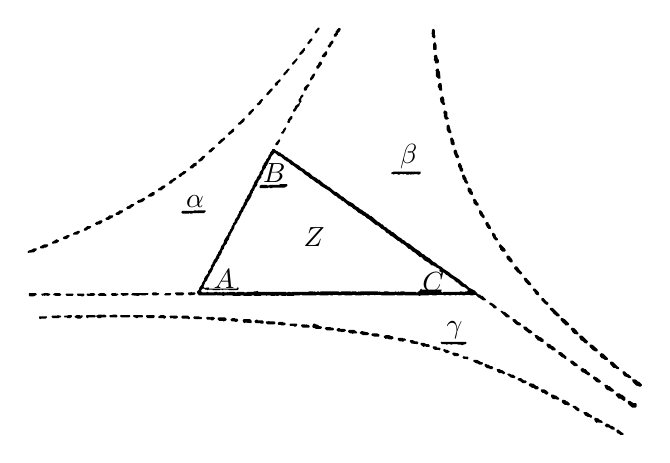
\begin{tikzpicture}[x=0.00720072cm,y=-0.00720072cm]
\fill[even odd rule] (1051,736) -- (1052,739) -- (1054,741) -- (1056,741) -- (1058,743) -- (1063,743) -- (1064,742) -- (1064,741) -- (1062,739) -- (1061,739) -- (1055,734) -- (1053,734) -- cycle
(1031,726) -- (1031,727) -- (1034,730) -- (1038,730) -- (1044,734) -- (1047,734) -- (1048,733) -- (1048,730) -- (1043,727) -- (1041,727) -- (1039,725) -- (1034,723) -- cycle
(1012,715) -- (1013,719) -- (1016,722) -- (1018,721) -- (1026,722) -- (1027,721) -- (1027,720) -- (1024,717) -- (1022,717) -- (1019,714) -- (1014,713) -- cycle
(993,704) -- (996,709) -- (1000,711) -- (1005,712) -- (1006,713) -- (1008,712) -- (1008,709) -- (999,703) -- (994,703) -- cycle
(974,693) -- (974,694) -- (982,701) -- (985,701) -- (986,700) -- (986,697) -- (979,692) -- (975,692) -- cycle
(1071,685) -- (1072,689) -- (1079,695) -- (1085,695) -- (1087,693) -- (1087,689) -- (1085,687) -- (1081,687) -- (1075,683) -- (1073,683) -- cycle
(955,683) -- (955,686) -- (960,690) -- (964,690) -- (965,691) -- (967,691) -- (969,689) -- (969,688) -- (965,684) -- (963,684) -- (961,682) -- (957,681) -- cycle
(936,673) -- (936,676) -- (939,680) -- (945,680) -- (946,681) -- (949,681) -- (950,680) -- (950,678) -- (945,674) -- (941,673) -- (940,672) -- (937,672) -- cycle
(1050,672) -- (1050,673) -- (1055,679) -- (1058,679) -- (1064,683) -- (1065,683) -- (1067,681) -- (1067,677) -- (1061,672) -- (1059,672) -- (1057,670) -- (1052,670) -- cycle
(918,664) -- (918,666) -- (921,669) -- (923,669) -- (927,672) -- (929,672) -- (931,670) -- (931,668) -- (928,665) -- (924,663) -- (919,663) -- cycle
(1030,656) -- (1032,661) -- (1035,664) -- (1039,665) -- (1042,667) -- (1045,667) -- (1047,665) -- (1047,664) -- (1039,657) -- (1037,657) -- (1035,655) -- (1031,655) -- cycle
(897,654) -- (897,656) -- (899,658) -- (900,658) -- (902,660) -- (905,660) -- (909,663) -- (912,663) -- (914,661) -- (914,659) -- (912,657) -- (910,657) -- (905,653) -- (899,652) -- cycle
(1079,646) -- (1080,650) -- (1086,656) -- (1090,657) -- (1091,658) -- (1094,658) -- (1096,656) -- (1096,654) -- (1091,649) -- (1089,649) -- (1086,646) -- (1084,645) -- (1080,645) -- cycle
(877,645) -- (878,647) -- (881,648) -- (886,652) -- (890,652) -- (893,650) -- (893,649) -- (891,647) -- (888,647) -- (883,643) -- (879,643) -- cycle
(1010,642) -- (1010,644) -- (1016,650) -- (1021,651) -- (1024,649) -- (1024,648) -- (1017,642) -- (1012,640) -- cycle
(859,636) -- (859,637) -- (865,642) -- (871,643) -- (873,641) -- (873,640) -- (869,637) -- (866,637) -- (863,635) -- (860,635) -- cycle
(1062,632) -- (1062,634) -- (1064,638) -- (1066,640) -- (1070,641) -- (1073,643) -- (1076,643) -- (1077,642) -- (1077,640) -- (1072,636) -- (1071,636) -- (1066,631) -- (1063,631) -- cycle
(840,628) -- (841,631) -- (844,634) -- (849,634) -- (852,636) -- (853,636) -- (855,634) -- (855,633) -- (850,629) -- (848,629) -- (845,627) -- (841,627) -- cycle
(988,627) -- (988,629) -- (991,633) -- (993,633) -- (1001,638) -- (1003,638) -- (1005,636) -- (1005,635) -- (1002,632) -- (1001,632) -- (997,627) -- (995,627) -- (992,625) -- cycle
(819,619) -- (819,622) -- (821,624) -- (825,626) -- (827,626) -- (828,627) -- (832,627) -- (834,625) -- (834,624) -- (832,622) -- (829,622) -- (825,619) -- (823,619) -- (822,618) -- (820,618) -- cycle
(1040,615) -- (1040,618) -- (1046,625) -- (1049,625) -- (1052,627) -- (1055,627) -- (1056,626) -- (1056,624) -- (1054,623) -- (1046,615) -- (1044,614) -- (1041,614) -- cycle
(970,613) -- (970,616) -- (977,622) -- (982,622) -- (983,621) -- (983,619) -- (974,612) -- (971,612) -- cycle
(799,612) -- (799,614) -- (804,617) -- (806,617) -- (809,619) -- (814,619) -- (816,617) -- (815,615) -- (813,615) -- (806,611) -- (800,611) -- cycle
(780,606) -- (780,607) -- (782,609) -- (786,609) -- (788,610) -- (790,608) -- (790,606) -- (789,605) -- (784,605) -- (782,604) -- cycle
(1022,601) -- (1022,604) -- (1025,608) -- (1027,608) -- (1031,611) -- (1035,611) -- (1036,610) -- (1036,608) -- (1028,600) -- (1025,599) -- cycle
(762,599) -- (762,601) -- (765,604) -- (772,604) -- (774,602) -- (774,601) -- (771,599) -- (768,599) -- (767,598) -- (763,598) -- cycle
(949,598) -- (949,601) -- (955,606) -- (958,607) -- (960,609) -- (962,609) -- (963,608) -- (963,605) -- (955,598) -- (953,597) -- (950,597) -- cycle
(746,593) -- (746,595) -- (751,599) -- (753,599) -- (757,597) -- (757,596) -- (753,593) -- (750,593) -- (749,592) -- (747,592) -- cycle
(727,588) -- (728,591) -- (731,593) -- (737,593) -- (739,594) -- (741,592) -- (741,591) -- (739,589) -- (735,589) -- (733,587) -- (728,587) -- cycle
(1004,585) -- (1004,588) -- (1010,594) -- (1014,596) -- (1017,596) -- (1018,595) -- (1018,592) -- (1010,585) -- (1008,584) -- (1005,584) -- cycle
(928,583) -- (928,586) -- (931,590) -- (935,591) -- (938,594) -- (943,594) -- (944,593) -- (944,591) -- (940,587) -- (937,586) -- (934,583) -- (932,583) -- (931,582) -- (929,582) -- cycle
(706,582) -- (706,584) -- (711,588) -- (713,587) -- (715,587) -- (716,588) -- (721,588) -- (722,587) -- (722,585) -- (720,583) -- (716,583) -- (712,581) -- (707,581) -- cycle
(741,579) -- (743,583) -- (750,583) -- (751,584) -- (753,584) -- (754,583) -- (758,583) -- (759,584) -- (761,584) -- (762,583) -- (771,583) -- (772,584) -- (777,584) -- (778,585) -- (780,585) -- (781,584) -- (785,583) -- (787,581) -- (786,579) -- cycle
(687,577) -- (687,579) -- (690,582) -- (700,583) -- (702,581) -- (701,579) -- (699,578) -- (696,578) -- (692,576) -- (688,576) -- cycle
(666,573) -- (666,576) -- (669,578) -- (673,578) -- (675,579) -- (677,577) -- (679,577) -- (680,576) -- (680,575) -- (678,573) -- (675,573) -- (674,572) -- (667,572) -- cycle
(987,568) -- (986,569) -- (986,572) -- (988,576) -- (992,578) -- (995,581) -- (998,582) -- (1001,579) -- (1001,578) -- (992,569) -- (990,568) -- cycle
(907,568) -- (908,571) -- (913,577) -- (915,577) -- (918,579) -- (922,579) -- (923,578) -- (923,575) -- (918,571) -- (915,570) -- (911,567) -- (908,567) -- cycle
(641,569) -- (641,571) -- (644,574) -- (647,573) -- (648,574) -- (654,575) -- (658,573) -- (658,571) -- (656,569) -- (654,569) -- (650,567) -- (645,567) -- cycle
(619,566) -- (619,567) -- (621,569) -- (623,569) -- (624,570) -- (632,570) -- (633,569) -- (633,566) -- (629,564) -- (621,564) -- cycle
(599,562) -- (599,564) -- (604,567) -- (613,567) -- (615,565) -- (615,564) -- (612,562) -- (609,562) -- (608,561) -- (605,561) -- (604,560) -- (602,560) -- cycle
(578,560) -- (578,561) -- (580,563) -- (582,564) -- (585,564) -- (586,565) -- (588,564) -- (593,564) -- (594,563) -- (594,562) -- (589,558) -- (580,558) -- cycle
(558,557) -- (558,559) -- (561,561) -- (565,561) -- (566,562) -- (572,561) -- (574,559) -- (574,558) -- (571,556) -- (564,556) -- (563,555) -- (560,555) -- cycle
(973,554) -- (971,556) -- (971,558) -- (973,560) -- (973,561) -- (977,565) -- (983,566) -- (984,565) -- (984,563) -- (982,561) -- (982,560) -- (977,555) -- cycle
(537,555) -- (537,556) -- (541,559) -- (551,559) -- (553,557) -- (553,556) -- (551,554) -- (548,554) -- (547,553) -- (539,553) -- cycle
(887,553) -- (888,557) -- (897,564) -- (900,564) -- (903,562) -- (903,561) -- (901,559) -- (897,557) -- (892,552) -- (888,552) -- cycle
(495,550) -- (495,551) -- (498,554) -- (509,554) -- (510,553) -- (510,551) -- (508,549) -- (506,549) -- (505,548) -- (503,549) -- (501,548) -- (497,548) -- cycle
(515,551) -- (515,553) -- (517,555) -- (520,555) -- (521,556) -- (530,556) -- (532,554) -- (531,552) -- (527,551) -- (525,549) -- (521,548) -- (520,547) -- (517,547) -- cycle
(475,548) -- (475,550) -- (476,551) -- (482,551) -- (483,552) -- (486,552) -- (488,550) -- (488,548) -- (487,547) -- (476,547) -- cycle
(454,546) -- (454,548) -- (455,549) -- (459,549) -- (460,550) -- (465,550) -- (468,548) -- (468,547) -- (466,545) -- (464,545) -- (463,544) -- (456,544) -- cycle
(433,544) -- (433,546) -- (436,548) -- (448,548) -- (450,546) -- (450,545) -- (448,543) -- (440,543) -- (438,542) -- (437,543) -- (434,543) -- cycle
(413,542) -- (413,544) -- (415,546) -- (423,546) -- (424,547) -- (428,547) -- (429,546) -- (429,543) -- (427,541) -- (419,541) -- (418,540) -- (416,540) -- cycle
(868,540) -- (868,542) -- (874,548) -- (878,550) -- (881,550) -- (883,548) -- (883,547) -- (881,545) -- (878,544) -- (873,539) -- (869,539) -- cycle
(392,541) -- (393,544) -- (395,546) -- (397,545) -- (407,546) -- (408,545) -- (408,542) -- (405,539) -- (394,539) -- cycle
(953,538) -- (953,541) -- (955,543) -- (955,544) -- (960,548) -- (961,550) -- (966,550) -- (968,548) -- (968,547) -- (960,539) -- (959,539) -- (957,537) -- (954,537) -- cycle
(371,539) -- (371,541) -- (373,543) -- (378,543) -- (379,544) -- (381,544) -- (384,542) -- (384,540) -- (382,538) -- (379,538) -- (378,537) -- (375,537) -- cycle
(348,538) -- (348,539) -- (351,542) -- (357,542) -- (358,543) -- (362,542) -- (364,540) -- (364,539) -- (361,536) -- (350,536) -- cycle
(328,536) -- (328,538) -- (330,540) -- (336,540) -- (337,541) -- (340,541) -- (343,538) -- (343,537) -- (340,535) -- (336,535) -- (335,536) -- (333,535) -- (329,535) -- cycle
(305,536) -- (305,537) -- (308,539) -- (319,539) -- (320,538) -- (320,536) -- (319,535) -- (316,535) -- (315,534) -- (307,534) -- cycle
(33,535) -- (33,537) -- (35,539) -- (37,538) -- (45,538) -- (47,536) -- (47,534) -- (34,534) -- cycle
(284,535) -- (284,536) -- (286,538) -- (295,538) -- (296,539) -- (298,539) -- (299,538) -- (299,536) -- (296,533) -- (286,533) -- cycle
(263,534) -- (265,538) -- (267,537) -- (269,537) -- (270,538) -- (275,538) -- (278,536) -- (278,535) -- (276,533) -- (264,533) -- cycle
(243,535) -- (244,537) -- (252,537) -- (253,538) -- (255,538) -- (257,536) -- (257,534) -- (253,532) -- (247,532) -- cycle
(222,533) -- (222,535) -- (224,537) -- (235,537) -- (237,535) -- (237,533) -- (236,532) -- (223,532) -- cycle
(199,533) -- (199,534) -- (201,536) -- (203,536) -- (204,537) -- (207,537) -- (208,536) -- (215,536) -- (216,535) -- (216,533) -- (215,532) -- (200,532) -- cycle
(176,533) -- (176,534) -- (178,536) -- (192,536) -- (194,534) -- (193,532) -- (177,532) -- cycle
(96,534) -- (96,535) -- (98,537) -- (100,537) -- (101,538) -- (106,538) -- (110,535) -- (110,533) -- (109,532) -- (107,533) -- (105,532) -- (99,532) -- cycle
(91,533) -- (90,532) -- (84,532) -- (83,533) -- (78,533) -- (77,535) -- (78,536) -- (82,536) -- (83,537) -- (88,537) -- (91,535) -- cycle
(72,534) -- (71,533) -- (66,532) -- (65,533) -- (56,533) -- (55,535) -- (57,537) -- (68,537) -- (69,536) -- (71,536) -- cycle
(157,533) -- (157,534) -- (159,536) -- (170,536) -- (171,535) -- (171,533) -- (169,531) -- (163,531) -- (162,532) -- (158,532) -- cycle
(152,533) -- (148,531) -- (146,531) -- (145,532) -- (143,531) -- (138,531) -- (134,533) -- (132,533) -- (131,532) -- (117,532) -- (116,533) -- (116,535) -- (118,537) -- (119,537) -- (120,536) -- (131,536) -- (133,534) -- (134,534) -- (137,537) -- (142,537) -- (143,536) -- (150,536) -- (152,534) -- cycle
(847,525) -- (847,526) -- (857,536) -- (862,536) -- (863,535) -- (863,533) -- (854,526) -- (852,526) -- (849,524) -- cycle
(934,520) -- (934,522) -- (939,527) -- (939,528) -- (946,534) -- (950,534) -- (951,533) -- (951,531) -- (939,519) -- (935,519) -- cycle
(827,511) -- (827,513) -- (832,516) -- (835,520) -- (839,520) -- (840,519) -- (840,517) -- (834,512) -- (830,510) -- (828,510) -- cycle
(920,502) -- (919,503) -- (919,506) -- (925,512) -- (929,514) -- (931,512) -- (931,510) -- (929,508) -- (928,508) -- (923,502) -- cycle
(100,495) -- (100,496) -- (102,498) -- (107,498) -- (108,499) -- (110,499) -- (113,497) -- (113,495) -- (112,494) -- (101,494) -- cycle
(80,495) -- (80,496) -- (82,498) -- (92,498) -- (94,496) -- (93,494) -- (81,494) -- cycle
(254,496) -- (255,497) -- (264,497) -- (266,495) -- (266,494) -- (265,493) -- (256,493) -- (254,495) -- cycle
(196,496) -- (197,497) -- (208,498) -- (212,496) -- (214,497) -- (221,497) -- (222,496) -- (225,496) -- (226,494) -- (225,493) -- (198,493) -- (196,495) -- cycle
(177,494) -- (177,495) -- (181,498) -- (189,497) -- (191,495) -- (190,493) -- (178,493) -- cycle
(160,495) -- (160,496) -- (162,498) -- (169,498) -- (173,496) -- (172,494) -- (169,494) -- (168,493) -- (162,493) -- cycle
(137,495) -- (137,496) -- (139,498) -- (151,498) -- (152,497) -- (152,496) -- (148,493) -- (141,493) -- cycle
(117,495) -- (117,496) -- (119,498) -- (129,498) -- (132,496) -- (132,495) -- (130,493) -- (124,493) -- (123,494) -- (118,494) -- cycle
(58,495) -- (59,497) -- (61,497) -- (62,498) -- (70,498) -- (72,496) -- (72,495) -- (69,493) -- (61,493) -- cycle
(37,495) -- (37,496) -- (39,498) -- (41,497) -- (43,498) -- (45,497) -- (49,498) -- (53,496) -- (52,494) -- (50,494) -- (49,493) -- (42,493) -- (41,494) -- (38,494) -- cycle
(15,494) -- (15,497) -- (17,499) -- (23,499) -- (29,496) -- (29,495) -- (27,493) -- (16,493) -- cycle
(273,493) -- (273,494) -- (276,497) -- (286,497) -- (289,495) -- (289,494) -- (287,492) -- (274,492) -- cycle
(232,494) -- (232,495) -- (234,497) -- (241,497) -- (245,495) -- (244,493) -- (241,493) -- (240,492) -- (234,492) -- cycle
(296,493) -- (296,495) -- (299,497) -- (307,496) -- (309,494) -- (308,492) -- (303,492) -- (302,491) -- (300,492) -- (297,492) -- cycle
(905,485) -- (904,486) -- (904,488) -- (907,491) -- (907,493) -- (910,496) -- (913,497) -- (915,495) -- (914,491) -- (908,485) -- cycle
(889,466) -- (888,467) -- (888,469) -- (890,473) -- (896,479) -- (900,479) -- (901,478) -- (901,476) -- (892,466) -- cycle
(873,446) -- (871,448) -- (871,450) -- (877,457) -- (878,457) -- (881,460) -- (883,460) -- (885,458) -- (885,457) -- (880,452) -- (880,451) -- (876,446) -- cycle
(859,427) -- (857,429) -- (858,433) -- (864,439) -- (867,439) -- (868,438) -- (868,435) -- (867,433) -- (862,427) -- cycle
(29,415) -- (28,414) -- (24,414) -- (19,417) -- (15,418) -- (13,420) -- (13,421) -- (14,422) -- (24,421) -- (29,417) -- cycle
(846,407) -- (844,410) -- (844,412) -- (846,414) -- (846,416) -- (850,420) -- (854,420) -- (856,418) -- (855,415) -- (847,407) -- cycle
(49,408) -- (48,407) -- (42,407) -- (35,411) -- (35,413) -- (36,414) -- (41,414) -- (42,413) -- (45,413) -- (49,410) -- cycle
(68,400) -- (64,398) -- (56,403) -- (56,405) -- (57,406) -- (64,405) -- (68,402) -- cycle
(87,392) -- (86,391) -- (82,391) -- (76,394) -- (75,396) -- (77,398) -- (81,398) -- (83,397) -- (87,393) -- cycle
(833,387) -- (832,388) -- (832,391) -- (835,397) -- (838,400) -- (841,400) -- (842,399) -- (842,397) -- (839,394) -- (838,390) -- (835,387) -- cycle
(105,385) -- (103,383) -- (95,386) -- (93,388) -- (93,389) -- (94,390) -- (100,390) -- (102,389) -- (105,386) -- cycle
(125,376) -- (124,375) -- (118,375) -- (112,380) -- (112,382) -- (113,383) -- (116,383) -- (120,380) -- (123,379) -- (125,377) -- cycle
(822,368) -- (820,370) -- (820,371) -- (823,377) -- (826,380) -- (829,380) -- (830,379) -- (830,377) -- (828,373) -- (826,371) -- (826,369) -- (825,368) -- cycle
(145,366) -- (144,365) -- (140,365) -- (137,367) -- (135,367) -- (132,370) -- (132,371) -- (135,373) -- (137,372) -- (140,372) -- (144,369) -- cycle
(164,357) -- (163,356) -- (157,356) -- (154,359) -- (151,360) -- (150,362) -- (152,364) -- (156,364) -- (160,361) -- (162,361) -- cycle
(810,347) -- (809,348) -- (809,352) -- (811,356) -- (816,361) -- (817,361) -- (819,359) -- (819,357) -- (816,353) -- (815,350) -- (812,347) -- cycle
(327,348) -- (326,347) -- (313,347) -- (312,348) -- (310,347) -- (307,347) -- (306,348) -- (286,348) -- (284,350) -- (284,351) -- (286,353) -- (297,353) -- (298,352) -- (300,353) -- (303,353) -- (304,352) -- (324,352) -- (327,349) -- cycle
(181,348) -- (180,347) -- (175,347) -- (173,349) -- (168,352) -- (168,354) -- (169,355) -- (174,355) -- (176,353) -- (179,352) -- (181,350) -- cycle
(201,337) -- (200,336) -- (196,336) -- (192,339) -- (189,340) -- (187,342) -- (187,343) -- (189,345) -- (194,344) -- (197,341) -- (198,341) -- (201,338) -- cycle
(800,327) -- (798,329) -- (799,331) -- (799,334) -- (804,339) -- (807,339) -- (808,338) -- (808,335) -- (806,333) -- (804,329) -- (802,327) -- cycle
(220,327) -- (218,325) -- (217,325) -- (212,328) -- (208,329) -- (206,331) -- (206,332) -- (208,334) -- (213,333) -- (217,331) -- (220,328) -- cycle
(237,316) -- (236,315) -- (233,315) -- (228,318) -- (225,321) -- (225,322) -- (226,323) -- (231,323) -- (235,321) -- (237,319) -- cycle
(790,307) -- (789,308) -- (789,313) -- (793,319) -- (797,320) -- (798,319) -- (798,315) -- (796,312) -- (796,310) -- (792,307) -- cycle
(256,305) -- (254,303) -- (250,304) -- (248,306) -- (243,309) -- (243,311) -- (244,312) -- (249,312) -- (252,309) -- (253,309) -- (256,306) -- cycle
(275,291) -- (274,290) -- (271,290) -- (268,293) -- (266,293) -- (262,297) -- (262,299) -- (263,300) -- (266,300) -- (270,296) -- (275,293) -- cycle
(780,285) -- (779,286) -- (780,292) -- (782,294) -- (783,297) -- (786,300) -- (789,300) -- (790,298) -- (787,293) -- (787,291) -- (783,284) -- cycle
(654,281) -- (655,283) -- (657,283) -- (658,284) -- (660,283) -- (665,283) -- (666,284) -- (669,284) -- (670,283) -- (674,283) -- (675,284) -- (677,283) -- (680,283) -- (681,284) -- (685,284) -- (686,283) -- (688,284) -- (700,283) -- (701,284) -- (703,284) -- (706,282) -- (706,279) -- (658,279) -- cycle
(293,279) -- (292,278) -- (288,278) -- (283,282) -- (282,282) -- (279,285) -- (279,286) -- (281,288) -- (283,288) -- (286,285) -- (290,283) -- (293,280) -- cycle
(774,264) -- (772,266) -- (772,270) -- (774,273) -- (775,277) -- (777,279) -- (779,279) -- (781,277) -- (781,274) -- (779,272) -- (779,269) -- (776,264) -- cycle
(311,264) -- (310,263) -- (306,264) -- (299,270) -- (299,272) -- (300,273) -- (304,273) -- (308,269) -- (310,269) -- (311,268) -- cycle
(326,252) -- (325,251) -- (322,251) -- (316,257) -- (314,258) -- (314,260) -- (315,261) -- (317,261) -- (321,259) -- (326,253) -- cycle
(767,240) -- (764,242) -- (764,245) -- (768,254) -- (769,255) -- (772,255) -- (774,253) -- (774,252) -- (771,247) -- (770,242) -- (768,240) -- cycle
(312,490) -- (312,493) -- (315,497) -- (344,497) -- (346,496) -- (347,497) -- (356,497) -- (357,498) -- (359,498) -- (360,497) -- (374,497) -- (375,498) -- (388,498) -- (389,497) -- (393,497) -- (394,498) -- (407,498) -- (408,497) -- (412,497) -- (413,498) -- (424,498) -- (425,497) -- (433,497) -- (434,498) -- (436,497) -- (441,497) -- (442,498) -- (449,498) -- (450,497) -- (452,498) -- (455,498) -- (456,497) -- (460,497) -- (461,498) -- (468,498) -- (470,497) -- (471,498) -- (482,498) -- (483,497) -- (493,497) -- (494,496) -- (496,496) -- (497,497) -- (522,497) -- (523,496) -- (527,496) -- (528,497) -- (543,497) -- (544,496) -- (546,496) -- (547,497) -- (551,497) -- (552,496) -- (559,496) -- (560,497) -- (566,497) -- (567,496) -- (571,496) -- (572,497) -- (585,497) -- (586,496) -- (590,496) -- (591,497) -- (602,497) -- (603,496) -- (605,497) -- (607,496) -- (611,496) -- (612,497) -- (616,497) -- (617,496) -- (624,496) -- (625,497) -- (627,496) -- (636,496) -- (637,497) -- (660,497) -- (661,496) -- (663,496) -- (664,497) -- (675,497) -- (677,496) -- (678,497) -- (702,497) -- (703,498) -- (705,498) -- (706,497) -- (720,497) -- (721,496) -- (726,496) -- (727,497) -- (734,497) -- (735,496) -- (746,496) -- (747,497) -- (750,497) -- (751,496) -- (755,496) -- (756,497) -- (760,497) -- (761,496) -- (766,496) -- (767,497) -- (769,497) -- (770,496) -- (774,496) -- (775,497) -- (777,496) -- (779,496) -- (780,497) -- (784,497) -- (785,496) -- (793,496) -- (794,497) -- (799,497) -- (800,496) -- (803,496) -- (808,501) -- (809,501) -- (816,506) -- (820,506) -- (821,505) -- (821,504) -- (815,498) -- (813,498) -- (811,496) -- (807,495) -- (802,489) -- (792,484) -- (786,478) -- (783,477) -- (774,469) -- (760,460) -- (757,457) -- (746,450) -- (743,447) -- (737,444) -- (733,440) -- (727,437) -- (722,432) -- (715,428) -- (712,425) -- (709,424) -- (704,419) -- (697,415) -- (686,406) -- (681,404) -- (677,400) -- (674,399) -- (671,396) -- (667,394) -- (658,386) -- (655,385) -- (652,382) -- (649,381) -- (645,377) -- (642,376) -- (639,372) -- (637,372) -- (634,369) -- (630,367) -- (619,357) -- (617,357) -- (613,353) -- (611,353) -- (608,350) -- (607,350) -- (602,346) -- (599,345) -- (596,342) -- (592,340) -- (587,335) -- (577,330) -- (569,323) -- (566,322) -- (561,317) -- (560,317) -- (558,315) -- (554,314) -- (545,306) -- (542,305) -- (540,303) -- (536,301) -- (527,293) -- (525,293) -- (522,290) -- (516,287) -- (510,281) -- (505,279) -- (501,275) -- (495,272) -- (491,268) -- (484,264) -- (477,258) -- (474,257) -- (471,254) -- (468,253) -- (464,249) -- (461,248) -- (458,245) -- (456,245) -- (454,243) -- (451,242) -- (448,239) -- (445,239) -- (444,240) -- (444,241) -- (440,246) -- (440,248) -- (438,250) -- (437,254) -- (434,257) -- (433,260) -- (429,265) -- (429,267) -- (427,269) -- (426,275) -- (422,280) -- (422,282) -- (420,286) -- (418,288) -- (416,293) -- (414,295) -- (412,299) -- (412,301) -- (410,303) -- (409,307) -- (405,313) -- (404,317) -- (400,322) -- (399,326) -- (396,329) -- (396,332) -- (394,334) -- (394,336) -- (392,340) -- (390,342) -- (388,347) -- (386,349) -- (386,351) -- (383,356) -- (383,358) -- (380,361) -- (378,365) -- (378,367) -- (375,370) -- (375,372) -- (372,377) -- (372,379) -- (370,381) -- (369,384) -- (367,386) -- (366,390) -- (361,397) -- (359,401) -- (359,403) -- (357,407) -- (355,409) -- (352,417) -- (349,421) -- (349,423) -- (347,425) -- (344,432) -- (341,435) -- (341,437) -- (339,439) -- (339,441) -- (336,445) -- (336,448) -- (331,455) -- (331,458) -- (326,464) -- (324,468) -- (324,470) -- (320,476) -- (320,478) -- (316,483) -- (315,487) -- cycle
(319,490) -- (319,488) -- (322,485) -- (324,485) -- (326,487) -- (329,487) -- (330,488) -- (332,487) -- (339,487) -- (340,488) -- (351,488) -- (352,487) -- (355,487) -- (356,488) -- (358,487) -- (367,487) -- (368,488) -- (383,488) -- (385,486) -- (385,484) -- (384,483) -- (383,483) -- (382,485) -- (333,485) -- (332,483) -- (325,484) -- (323,482) -- (326,474) -- (330,470) -- (330,468) -- (332,464) -- (334,462) -- (334,460) -- (337,456) -- (340,450) -- (340,448) -- (343,444) -- (343,442) -- (348,436) -- (348,434) -- (351,431) -- (351,428) -- (353,426) -- (356,420) -- (356,418) -- (359,415) -- (360,410) -- (364,406) -- (365,402) -- (368,398) -- (369,393) -- (371,391) -- (371,389) -- (377,379) -- (378,374) -- (383,368) -- (383,366) -- (386,362) -- (391,351) -- (393,349) -- (394,345) -- (396,343) -- (397,340) -- (400,336) -- (400,334) -- (405,327) -- (408,321) -- (408,319) -- (410,316) -- (410,314) -- (412,312) -- (414,307) -- (417,304) -- (418,302) -- (418,299) -- (420,297) -- (420,295) -- (425,289) -- (425,286) -- (428,282) -- (429,277) -- (433,272) -- (433,270) -- (435,268) -- (439,259) -- (441,257) -- (442,253) -- (448,246) -- (451,247) -- (455,251) -- (459,252) -- (467,259) -- (468,259) -- (470,261) -- (472,261) -- (478,267) -- (481,268) -- (491,276) -- (496,278) -- (502,284) -- (507,287) -- (511,291) -- (514,292) -- (523,299) -- (526,300) -- (530,304) -- (545,313) -- (554,321) -- (557,322) -- (561,326) -- (564,327) -- (568,331) -- (570,331) -- (579,339) -- (584,341) -- (588,345) -- (591,346) -- (596,351) -- (602,354) -- (604,356) -- (607,357) -- (611,361) -- (615,363) -- (627,373) -- (631,374) -- (636,379) -- (642,382) -- (646,387) -- (649,388) -- (653,392) -- (656,393) -- (666,401) -- (669,402) -- (673,406) -- (675,406) -- (677,408) -- (678,408) -- (685,415) -- (687,415) -- (692,420) -- (695,421) -- (704,429) -- (708,430) -- (712,435) -- (720,439) -- (725,444) -- (728,444) -- (730,446) -- (732,446) -- (734,448) -- (737,449) -- (740,452) -- (739,454) -- (740,455) -- (741,455) -- (743,457) -- (744,456) -- (747,457) -- (751,461) -- (754,462) -- (757,465) -- (764,469) -- (769,474) -- (771,474) -- (778,481) -- (784,483) -- (789,487) -- (789,489) -- (788,490) -- (785,490) -- (784,491) -- (776,490) -- (775,491) -- (746,491) -- (745,492) -- (744,492) -- (742,490) -- (743,487) -- (708,487) -- (707,485) -- (705,487) -- (705,488) -- (700,492) -- (698,492) -- (697,491) -- (678,491) -- (677,490) -- (671,490) -- (670,491) -- (668,491) -- (667,490) -- (665,491) -- (663,491) -- (662,490) -- (660,491) -- (650,491) -- (649,490) -- (642,490) -- (641,491) -- (635,491) -- (634,490) -- (632,491) -- (630,490) -- (600,490) -- (599,491) -- (597,490) -- (595,491) -- (593,491) -- (592,490) -- (585,490) -- (584,491) -- (582,490) -- (566,490) -- (565,491) -- (562,491) -- (561,490) -- (530,490) -- (529,491) -- (527,491) -- (526,490) -- (524,490) -- (523,491) -- (521,491) -- (519,490) -- (517,491) -- (516,490) -- (509,490) -- (508,491) -- (479,491) -- (478,492) -- (476,491) -- (472,491) -- (471,492) -- (469,492) -- (468,491) -- (420,491) -- (418,489) -- (416,490) -- (412,490) -- (411,491) -- (400,491) -- (399,492) -- (395,492) -- (394,491) -- (383,491) -- (382,492) -- (379,492) -- (378,491) -- (369,491) -- (368,492) -- (366,491) -- (364,492) -- (360,492) -- (359,491) -- (357,491) -- (356,492) -- (353,492) -- (352,491) -- (350,492) -- (348,492) -- (347,491) -- (343,491) -- (342,492) -- (332,492) -- (331,491) -- (329,491) -- (328,492) -- (321,492) -- cycle
(471,302) -- (470,301) -- (458,301) -- (457,302) -- (440,302) -- (439,303) -- (435,303) -- (434,302) -- (425,302) -- (422,304) -- (422,307) -- (423,308) -- (436,308) -- (437,307) -- (440,307) -- (441,308) -- (444,308) -- (445,307) -- (466,307) -- (471,304) -- cycle
(343,237) -- (342,236) -- (339,236) -- (332,242) -- (332,244) -- (333,245) -- (336,245) -- (343,238) -- cycle
(457,222) -- (456,222) -- (450,229) -- (450,231) -- (451,232) -- (454,232) -- (458,225) -- (458,223) -- cycle
(760,219) -- (758,221) -- (759,229) -- (761,232) -- (765,232) -- (766,231) -- (766,227) -- (765,226) -- (765,224) -- (762,219) -- cycle
(361,220) -- (360,219) -- (358,219) -- (356,221) -- (355,221) -- (349,227) -- (349,229) -- (350,230) -- (352,230) -- (361,222) -- cycle
(376,203) -- (375,203) -- (366,211) -- (366,212) -- (368,214) -- (369,214) -- (377,208) -- (377,204) -- cycle
(468,201) -- (467,201) -- (464,204) -- (463,207) -- (460,210) -- (461,212) -- (464,212) -- (469,203) -- cycle
(754,196) -- (752,198) -- (752,205) -- (754,209) -- (756,211) -- (759,211) -- (760,210) -- (760,207) -- (759,206) -- (757,198) -- (755,196) -- cycle
(396,186) -- (395,185) -- (393,185) -- (386,192) -- (384,193) -- (384,195) -- (385,196) -- (388,196) -- (395,190) -- cycle
(479,181) -- (477,181) -- (472,187) -- (472,189) -- (471,190) -- (471,192) -- (472,193) -- (474,193) -- (476,191) -- (476,189) -- (479,186) -- (480,184) -- (480,182) -- cycle
(748,171) -- (746,174) -- (746,176) -- (747,177) -- (747,182) -- (748,183) -- (748,185) -- (750,187) -- (753,187) -- (756,185) -- (753,182) -- (753,174) -- (751,172) -- cycle
(411,168) -- (410,168) -- (403,174) -- (402,176) -- (402,178) -- (403,179) -- (405,179) -- (412,171) -- (412,169) -- cycle
(427,151) -- (425,151) -- (421,155) -- (421,156) -- (417,159) -- (417,160) -- (419,162) -- (422,161) -- (425,158) -- (426,155) -- (428,153) -- cycle
(742,147) -- (740,150) -- (741,156) -- (745,161) -- (748,161) -- (749,160) -- (749,158) -- (748,157) -- (748,151) -- (747,150) -- (747,148) -- (745,146) -- cycle
(498,143) -- (497,143) -- (494,146) -- (493,149) -- (491,151) -- (491,155) -- (492,156) -- (492,158) -- (485,163) -- (483,168) -- (481,170) -- (481,172) -- (482,173) -- (484,173) -- (486,171) -- (488,167) -- (492,163) -- (493,159) -- (496,155) -- (495,153) -- (496,149) -- (499,146) -- (499,144) -- cycle
(444,132) -- (441,133) -- (434,141) -- (434,143) -- (435,144) -- (437,144) -- (445,135) -- (445,133) -- cycle
(509,125) -- (506,125) -- (501,130) -- (500,132) -- (500,135) -- (501,136) -- (504,136) -- (506,134) -- (506,132) -- (510,127) -- cycle
(739,123) -- (737,125) -- (736,129) -- (738,132) -- (738,134) -- (740,136) -- (743,136) -- (744,135) -- (743,124) -- (742,123) -- cycle
(458,116) -- (457,116) -- (449,123) -- (449,126) -- (450,127) -- (453,127) -- (454,126) -- (454,124) -- (459,119) -- (459,117) -- cycle
(519,106) -- (517,106) -- (514,109) -- (513,112) -- (511,114) -- (511,117) -- (512,118) -- (513,118) -- (517,114) -- (520,108) -- cycle
(735,97) -- (732,100) -- (733,102) -- (733,111) -- (737,115) -- (740,115) -- (741,114) -- (740,103) -- (738,100) -- (738,98) -- (737,97) -- cycle
(474,97) -- (472,97) -- (464,106) -- (464,108) -- (465,109) -- (466,109) -- (472,103) -- (472,102) -- (475,99) -- cycle
(530,85) -- (528,85) -- (526,87) -- (525,90) -- (522,93) -- (522,96) -- (523,97) -- (526,97) -- (532,89) -- (532,87) -- cycle
(488,79) -- (487,79) -- (480,86) -- (479,88) -- (480,90) -- (482,90) -- (488,83) -- (489,81) -- cycle
(731,73) -- (729,76) -- (730,78) -- (729,82) -- (731,84) -- (731,87) -- (732,88) -- (736,88) -- (738,86) -- (738,82) -- (736,79) -- (735,74) -- (734,73) -- cycle
(540,67) -- (538,67) -- (532,74) -- (532,76) -- (533,77) -- (537,77) -- (541,72) -- (541,68) -- cycle
(501,61) -- (500,61) -- (492,70) -- (492,72) -- (493,73) -- (496,72) -- (500,68) -- (500,67) -- (502,65) -- (502,62) -- cycle
(730,51) -- (728,54) -- (728,63) -- (729,64) -- (733,64) -- (734,63) -- (734,55) -- (733,54) -- (733,52) -- (732,51) -- cycle
(551,48) -- (549,48) -- (545,52) -- (545,54) -- (542,57) -- (542,58) -- (544,60) -- (546,60) -- (548,58) -- (549,55) -- (552,52) -- (552,49) -- cycle
(514,44) -- (511,45) -- (506,52) -- (507,54) -- (509,54) -- (515,47) -- (515,45) -- cycle
(728,27) -- (726,29) -- (726,33) -- (725,35) -- (726,36) -- (726,41) -- (729,44) -- (730,44) -- (732,42) -- (732,39) -- (731,38) -- (731,30) -- (730,28) -- cycle
(564,26) -- (561,26) -- (558,29) -- (558,30) -- (556,32) -- (556,34) -- (553,37) -- (553,40) -- (554,41) -- (557,41) -- (558,40) -- (558,39) -- (560,37) -- (560,35) -- (563,32) -- (565,28) -- cycle
(527,25) -- (525,25) -- (520,31) -- (519,33) -- (520,35) -- (522,35) -- (524,33) -- (524,32) -- (528,27) -- cycle;
\node[inner sep=0pt] at (359,468) {$A$};
\node[inner sep=0pt] at (448,282) {$B$};
\node[inner sep=0pt] at (728,474) {$C$};
\node[inner sep=0pt] at (518,395) {$Z$};
\node[inner sep=0pt] at (308,331) {$\alpha$};
\node[inner sep=0pt] at (685,252) {$\beta$};
\node[inner sep=0pt] at (766,559) {$\gamma$};
\end{tikzpicture}
\end{center}

